\section{Aufbau}
    Im Folgenden wird der Aufbau des Algoritmus näher beschrieben. 
    Nach einem kurzem Überblick werden die einzelnen Subsysteme detailiert erklärt.
    \subsection{Grundlegende Struktur}
    % oberflächliche Beschreibung des systems
    Die oberflächliche Struktur des Generators ist im unteren Flussdiagram dargestellt. 
    Für eine gegebene Anzahl an Layern in einer Rota wird für jedes Layer folgedne Routine ausgeführt:
    \begin{itemize}
        \item wähle einen Modus, gewichtet nach den Mode-Wahrscheinlichkeiten und dem Mode-Spacing
        \item für den gewählten Modus werden die validen Maps gefiltert
        \begin{itemize}
            \item zunächst wird geprüft welche Map im Modus repräsentiert ist
            \item aus den vorhanden Maps wird nach dem Distanz-Vote-Weight $w_m$ gewichtet eine Map gezogen
        \end{itemize}
        \item für die gezogene Map wird gewichtet nach dem Layerweight $w_l$ ein Layer gezogen
        \item die gezogenen Maps verbleiben für eine feste Maplänge im Memory-Kernel und sind damit für die nächsten Map Ziehungen nicht verfügbar
    \end{itemize}
    \subsection{Aufbau im Detail - Mode}
        Wie zuvor erwähnt gibt es zwei Faktoren die die Ziehung des Modus beeinflussen:
        \begin{itemize}
            \item [1.] die Modeweights die zuvor gesetzt wurden $w_g$ 
            \item [2.] das Modespacing
        \end{itemize}
        Desweiteren erlaubt der Generator eine Gruppierung der Modes in soganennte ''Pools''. 
        Es gibt immer einen sogenannten \textit{main}-Pool. 
        Ohne weitere Einstellungen ist erstmal jeder Modus der gespielt werden soll damit automatisch im Main-Pool enthalten. 
        Neben diesem können noch händisch weitere Pools definiert werden. 
        In der momentanen Fassung existieren drei Pools:
        \begin{itemize}
            \item \textbf{main}: Der zuvor erwähnte Standard-Pool, beinhaltet \textit{RAAS} und \textit{AAS}
            \item \textbf{intermediates}: Beinhaltet die Modi \textit{Invasion} und \textit{TC}
            \item \textbf{reste}: Beinhaltet \textit{Destruction} und \textit{Insurgency}
        \end{itemize}
        Das \textbf{Modespacing} sorgt nun dafür dass für eine gegebene Anzahl an Runden nur der Main-Pool gezogen werden darf.
        Mit anderen Worten kann durch das Modespacing eine Mindestzeit definiert werden in der es nur Main-Modi geben kann. 
        Sollte die Zeitspanne seit dem letzten nicht-main Modus größer sein als das Modespacing so wird mit den Pool und Mode-weights gewichtet ein Gamemode gewählt. 
        Hierbei wird erst der Pool ausgewählt und anschließend im Pool der Modus. 
        Es ist zu beachten dass dies dazu führen kann und wird, dass nicht direkt nach Ablauf des Modespacings ein andere Pool drankommen muss. 
        Das Design wurde mit Absicht so gewählt um repititive Modes zu verhindern.

    \subsection{Aufbau im Detail - Map}
    Jeder Map die im Modus enthalten ist wird ein Mapvoteweight $w_m$ und ein Distanzweight $w_d$ zugeordnet. 
    Aus dem Produktweight wird anschließend die Map gezogen. 
    Hier kommt noch hinzu dass die Distanzweights vom Memory-Kernel abhängen. 
    In der momentanen Implementierung bedeutet dies, dass eine Map welche in den letzten $k$ Runden gezogen wurde nicht nochmal dran kommen kann. 
    Effektiv heißt dies $w_d=0$ für diese Map. 
    Für den seltenen Fall dass keine Map verfügbar ist für einen Modus weil alle in Frage kommenden Maps zurzeit gesperrt sind wird der Modus in den sogenannten \textbf{Mode-Buffer} verlegt. 
    Dieser wird beim ziehen des nächsten Modus abgearbeitet. 
    Das bedeutet ein Modus wird "ge-queued" und kommt bei der nächst passenden Gelgenheit dran. 
    
    \subsection{Aufbau im Detail - Layer}
    Sobald eine Map ausgewählt wurde wird das Layer gewichtet nach dem Layerweights $w_l$ gezogen. 
    Diese hängen nur von den Mapvotes ab welche mit der vorher genannten Sigmoidfunktion moduliert werden. 
    \begin{figure}[htbp]
        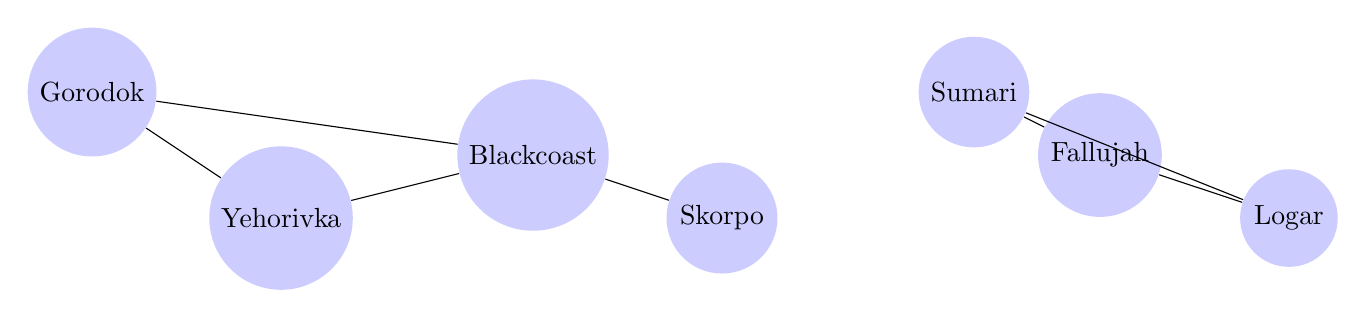
\begin{tikzpicture}
            [scale=.8,auto=left,every node/.style={circle,fill=blue!20}]
            \node (n1) at (1,10) {Gorodok};
            \node (n2) at (4,8)  {Yehorivka};
            \node (n3) at (8,9)  {Blackcoast};
            \node (n4) at (11,8) {Skorpo};
            \node (n5) at (15,10) {Sumari};
            \node (n6) at (20,8)  {Logar};
            \node (n7) at (17,9)  {Fallujah};
            \foreach \from/\to in {n1/n2,n1/n3,n2/n3,n3/n4,n5/n6,n5/n7,n6/n7}
            \draw (\from) -- (\to);  
        \end{tikzpicture}
    \caption{Cluster}
    \end{figure}